\documentclass{article}
\usepackage[utf8]{inputenc}
\usepackage{amsmath}
\usepackage{amsfonts}
\usepackage{graphicx}
% \usepackage{fancyhdr}
\usepackage[margin=1.0in]{geometry}
% \pagestyle{fancy}
% \fancyhf{}
% \fancyhead[LE,RO]{Note: Fourier Optics TDUs}
% \fancyhead[RE,LO]{Physics 325, Winter 2020}

\title{Polarimeter Analysis}
\date{}
\author{Scott Wilkinson, Aydan Mckay, Andrew MacRae}

\begin{document}
\setcounter{section}{0}
\maketitle


\section{Calibrating and Correcting the Retardance of a Waveplate}
\subsection{Importance of Waveplate Calibration}
Our method involves rotating a quarter waveplate in front of a linear polarizer to extract the Stokes vectors of a beam of light. Since we are relatively insensitive to (polarization independant) losses, we can assume an ideal linear polarizer -- that is we can assume that the transmission of the orthogonally polarized light is negligibly small. However, we are likely not justified in assuming an ideal quarter waveplate. \\

Supposing even that we have narrowband (or even monochromatic) light, a waveplate will typically have a wavelength-dependant phase delay. For a quarter waveplate, the relative delay between its fast and slow axes is $\delta = \frac{2n+1}{2}\pi$, where $n$ is an integer. The wavelength dependance can be minimized for a so-called ``zero-order'' waveplate\footnote{Actually there are two classes of zero-order waveplates, ``true'' and ``effective'' zero order. For true zero order, the physical delay between a monochromatic beam two polarizations is $\lambda/4$. Since this is very hard to make, typically two orthogonally oriented waveplates with order $m$ and $m+1$ are cemented together, advancing the beam by $(m+1)$ and delaying by $m$ quarter wavelengths, which has the same effect at the precise wavelength.}, i.e. on for which $n=0$, is used. Even for zero-order waveplates however, there is still \textit{some} wavelength dependance and so we can not assume that we have a real QWP for all angles. 

A waveplate with fast axis horizontal will create a relative phase shift $\delta$ between the horizontal and vertical polarization components. If we are working with fully polarized states, the Jones formalism may be used and the corresponding Jones matrix is given by\footnote{There is also a global phase shift applied to both beams $e^{i\phi}$ which is equivalent to simple propagation over a distance $L = 2\pi\phi\lambda$. This is not relevant here. Also note that some author prefer to share the phase equally between the two polarizations so the each component gets a phase factor $e^{\pm i \delta/2}$.}

\begin{equation}
    \label{eq:def_jones_wp}
    \begin{pmatrix}E_h \\ E_v 
    \end{pmatrix} \rightarrow 
    \begin{pmatrix}
        1 & 0 \\ 
        0 & e^{i\delta}
    \end{pmatrix}
    \begin{pmatrix}E_h \\ E_v 
    \end{pmatrix} = 
    \begin{pmatrix}E_h \\ e^{i\delta}E_v 
    \end{pmatrix}
\end{equation}

\subsection{A Method for Measuring $\delta$}
A simple method to measure the phase delay $\delta$ is to rotate the waveplate in between two polarizers. The polarizers can either be crossed or parallel. Experimentally it may be easier to align cross polarizers since it is easier to measure a minimum than a maximum. Suppose that the first polarizer is aligned horizontally. Regardless of the input light, it will be completely polarized horizontally with some amplitude $E_0$ and intensity $I\propto \vert E_0\vert^2$. Since it is completely polarized, we may work in the simpler Jones formalism. The output field is then:

\begin{equation}
    \label{eq:calpol_input}
    \vec{E}_{out} = P_hW_{\delta,\theta}\vec E_{in} = 
    \begin{pmatrix}
        1 & 0 \\ 
        0 & 0
    \end{pmatrix}
    \begin{pmatrix}
        A & B \\ 
        C & D
    \end{pmatrix} 
    \begin{pmatrix}E_0 \\ 0
    \end{pmatrix}=
    A\vec{E}_{0}
\end{equation}

\noindent\ldots where $W_{\delta,\theta}$ is the matrix corresponding to a waveplate of phase shift $\delta$ rotated an angle $\theta$ with respect to the horizontal. The output intensity is then
\begin{equation}
    \label{eq:calpol_intense}
    I_\delta(\theta) = \vert A\vert^2I_0
\end{equation}

With crossed polarizers, the intensity is similarly
\begin{equation}
    \label{eq:calpol_intense_crossed}
    I_{\delta,\perp}(\theta) = \vert B\vert^2I_0
\end{equation}

The parameters $A$ and $B$ can be obtained via rotating the waveplate in equation \ref{eq:def_jones_wp}:

\begin{align}
    \label{eq:rot_wp}
    P_hW_{\delta,\theta} &= R(\theta)P_h W_{\delta,0} R(-\theta) \nonumber \\
                         &= 
                         \begin{pmatrix}
                             \cos\theta & -\sin\theta \\ 
                             \sin\theta & \cos\theta
                         \end{pmatrix}
                         \begin{pmatrix}
                             1 & 0 \\ 
                             0 & e^{i\delta}
                         \end{pmatrix} 
                         \begin{pmatrix}
                             \cos\theta & \sin\theta \\ 
                             -\sin\theta & \cos\theta
                         \end{pmatrix} \nonumber \\
                         & = \begin{pmatrix}
                             \cos^2\theta + \sin^2\theta e^{i\delta} & \cos\theta\sin\theta\left(1-e^{i\delta}\right)\\ 
                             \cos\theta\sin\theta\left(1-e^{i\delta}\right) &\sin^2\theta + \cos^2\theta e^{i\delta}
                         \end{pmatrix} 
\end{align}

\noindent Thus the intensity as a function of angle is:
\begin{equation}
    \label{eq:calpol_intense_mark2}
    I_{\delta}(\theta) = \left(\cos^4\theta + \sin^4\theta + 2\cos^2\theta\sin^2\theta\cos\delta\right)I_0
\end{equation}

\noindent Note that if $\delta = \frac{2n+1}{2}\pi$ (with integer $n$), then $I_{\delta}(\theta) = I_0$ which is interesting. If $\delta = n\pi$ then $I_{\delta}(\theta) = \left(\cos^2\theta - \sin^2\theta\right)^2 = \cos^22\theta$ and we have perfect ``visibility''. Note as well that with the crossed polarizer result we have $\vert B\vert^2 = \sin4\theta\sin\frac{\delta}{2}$

To extract the phase $\delta$, we may align the polarizers in our setup and observe the resultant trace. An example of this is shown in figure \ref{fig:cal_wp}. There will be maxima and minima which can be used to extract the phase: taking the derivative of equation \ref{eq:calpol_intense_mark2} with respect to $\theta$:

\begin{align}
    \label{eq:calpolderiv}
    \frac{d}{d\theta}I_{\delta}(\theta) &= \left[2\cos\delta\sin2\theta\cos2\theta-4\cos\theta\sin\theta\left(\cos^2\theta - \sin\theta^2\right)\right]I_0 \nonumber \\
                                        &= \left[\sin4\theta\left(\cos\delta -1\right)\right]I_0
\end{align}

Setting this to zero we have either that $\delta = 0$ (as a special case - recall $\delta$ is fixed) or that $\theta = \frac{n\pi}{4}$. For even n, the third term in equation \ref{eq:calpol_intense_mark2} vanishes and either the sine or cosine gives 1 (the other is 0). This is the maximum at $I=I_0$. For odd $n$ the result is a minimum. In this case $\sin\theta = \cos\theta = 1/\sqrt{2}$ and we have.

\begin{equation}
    \label{eq:calpol_min}
    \frac{I_{min}}{I_{max}} \equiv \eta = \frac{1+\cos\delta}{2}
\end{equation}

We can thus find the phase delay of a waveplate as:

\begin{equation}
    \label{eq:calpol_final}
    \boxed{\delta = \arccos\left(2\eta-1\right)}
\end{equation}


\begin{figure}[h]
    \caption{Using a red LED to calibrate our QWP. We find that for this wavelength ($\lambda \approx 630$~nm) we have a $\lambda/3.0$ plate! An overall phase of 0.69 rad was added to equation \ref{eq:calpol_intense_mark2} to match the trigger origin of the motor.}
    \label{fig:cal_wp}
    \begin{center}
        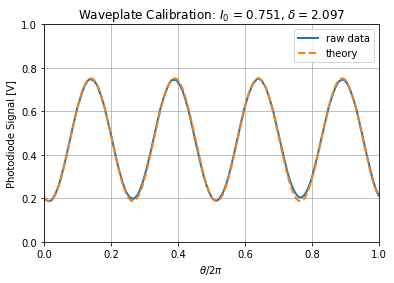
\includegraphics[width=0.45\textwidth]{wave_plate_cal}
    \end{center}
\end{figure}


\subsection{Correcting for Non-Ideal Waveplates}
Given that we know the true phase shift of our waveplate, can we still extract the Stokes parameters as before? It turns out that we can \ldots

\section{Expected Intensity, Given Stokes Vector}


\subsection{Mueller Matrix of our system}

Consider a monochromatic field with vacuum wavelength $\lambda$. A generic waveplate, with phase retardance $\delta/2$ and fast axis horizontal performs the transformation:

\begin{subequations}
    \begin{align}
        \label{eq:arb_wave_horiz}
        E_x &\rightarrow e^{i\delta/2} E_x \\
        E_y &\rightarrow e^{-i\delta/2} E_y
    \end{align}
\end{subequations}

Since $S_0 = \vert E_x\vert^2 + \vert E_y\vert^2$ and $S_1 = \vert E_x\vert^2 - \vert E_y\vert^2$, neither are affected by the waveplate as expected intuitively for a horizontal/vertical fast/slow axis. However, both $S_2$ and $S_3$ are affected. To see this, we can use Euler's identity:

\begin{align}
    S_2 &= E_xE_y^* + E_x^*E_y \nonumber \\
        &\rightarrow  e^{i\delta}E_xE_y^* + e^{-i\delta}E_x^*E_y \nonumber \\
        &= \cos\delta\left(E_xE_y^* + E_x^*E_y\right) + i\sin\delta\left(E_xE_y^* - E_x^*E_y\right)\nonumber \\
    S_2 &\rightarrow \cos\delta S_2 + \sin\delta S_3 \nonumber
\end{align}

Similarly, $S_3 \rightarrow \cos\delta S_3 - \sin\delta S_2$. Writing this as a matrix equation yeilds the Mueller matrix for a arbitrary waveplate:

\begin{equation}
    \label{eq:mueller_WPH}
    W_{\delta,0^\circ} = \begin{pmatrix}
        1 & 0 & 0 & 0 \\
        0 & 1 & 0 & 0 \\
        0 & 0 & \cos\delta & \sin\delta \\
        0 & 0 & -\sin\delta & \cos\delta 
    \end{pmatrix}
\end{equation}


To find the matrix corresponding to a waveplate rotated an angle $\theta$ to the horizontal we apply the rotation matrix\footnote{Note that the $2\theta$ comes about in taking the square to find the intensity.}:
\begin{equation}
    \label{eq:mueller_rot}
    R(\theta) = \begin{pmatrix}
        1 & 0 & 0 & 0 \\
        0 & \cos2\theta & -\sin2\theta & 0 \\
        0 &  \sin2\theta & \cos2\theta & 0 \\
        0 & 0 & 0 & 1
    \end{pmatrix}
\end{equation}

\noindent\ldots so that 
\begin{equation}
    \label{eq:mueller_rot_symb}
    W_{\delta,\theta} = R(\theta)W_{\delta,0^\circ}R(-\theta)
\end{equation}


The end result of this is then sent through a linear polarizer aligned horizontally, having matrix 

\begin{equation}
    \label{eq:mueller_pol0}
    P_0 = \frac{1}{2}\begin{pmatrix}
        1 & 1 & 0 & 0 \\
        1 & 1 & 0 & 0 \\
        0 & 0 & 0 & 0 \\
        0 & 0 & 0 & 0 
    \end{pmatrix}
\end{equation}

We can just blast away at the whole expression now but many of the terms will be redundant for our purposes. Recall that all we are measuring is the intensity, given by $S_0$. Note that, writing the rotated waveplate as some abstract matrix, we have that the stokes vector after passage through the system is

\begin{equation}
    \label{eq:sys_matrix_deriv1}
    \vec{S}^\prime = 
    \begin{pmatrix}
        I(\theta) \\
        S^\prime_1(\theta) \\
        S^\prime_2(\theta) \\
        S^\prime_3(\theta)
    \end{pmatrix}
    = 
    \frac{1}{2}
    \begin{pmatrix}
        1 & 1 & 0 & 0 \\
        1 & 1 & 0 & 0 \\
        0 & 0 & 0 & 0 \\
        0 & 0 & 0 & 0 
    \end{pmatrix}
    \begin{pmatrix}
        W_{11} & W_{12} & W_{13} & W_{14} \\
        W_{21} & W_{22} & W_{23} & W_{24} \\
        W_{31} & W_{32} & W_{33} & W_{34} \\
        W_{41} & W_{42} & W_{43} & W_{44}
    \end{pmatrix}
    \begin{pmatrix}
        S_0 \\
        S_1 \\
        S_2 \\
        S_3 
    \end{pmatrix} 
\end{equation}

From this, we can just take the first component of the output Stokes vector to find:
\begin{equation}
    \label{eq:Intense_theta_abs}
    I(\theta) = \frac{W_{11}+W_{21}}{2}S_0 + \frac{W_{12}+W_{22}}{2}S_1 + \frac{W_{13}+W_{23}}{2}S_2 + \frac{W_{41}+W_{24}}{2}S_3
\end{equation}

\noindent so we just need to find the first two rows of the rotated waveplate. Actually it isn't too much more work doing the whole calculation but this gives the answer in terms of what we calculate. Grinding out equation \ref{eq:mueller_rot_symb}, we get:

\begin{equation}
    \label{eq:mueller_rot_explicit}
    R(\theta) = \begin{pmatrix}
        1 & 0 & 0 & 0 \\
        0 & \cos^22\theta + \cos\delta\sin^22\theta & \sin2\theta\cos2\theta(1-\cos\delta) & -\sin2\theta\sin\delta \\
        0 &  \sin2\theta\cos2\theta(1-\cos\delta) & \sin^22\theta + \cos\delta\cos^22\theta & \cos2\theta\sin\delta \\
        0 & \sin\delta\sin2\theta & -\sin\delta\cos2\theta & \cos\delta
    \end{pmatrix}
\end{equation}

Finally, plugging this back into equation \ref{eq:Intense_theta_abs}, we have the desired result of the intensity as a function of Stokes parameters:

\begin{equation}
    \label{eq:Intense_theta_penultimate}
    I(\theta) = \frac{1}{2}S_0 + \frac{\cos^22\theta + \cos\delta\sin^22\theta}{2}S_1 + \frac{\sin2\theta\cos2\theta(1-\cos\delta)}{2}S_2 - \frac{\sin2\theta\sin\delta}{2}S_3
\end{equation}

Finally, by employing trigonometric half angle formulae ($\sin2x = 2\sin x\cos x$, $2\sin^2x = 1 - \cos2x$, and $2\cos^2x = 1 + \cos2x$) we arrive at:

\begin{equation}
    \label{eq:Intense_theta_ultimate}
    \boxed{I(\theta) = \frac{1}{2}\left[S_0 + \left(\frac{1+\cos\delta}{2}\right)S_1\right] - \left(\frac{\sin\delta}{2}S_3\right)\sin2\theta + \left(\frac{1-\cos\delta}{4}S_1\right)\cos4\theta + \left(\frac{1-\cos\delta}{4}S_2\right)\sin4\theta}
\end{equation}

Note that in the limit of an ideal quarter waveplate ($\delta = \pi/2$) this becomes

\begin{equation}
    \label{eq:Intense_theta_ultimate}
    I(\theta) =  \frac{2S_0+S_1}{4} - \frac{S_3}{2}\sin2\theta + \frac{S_1}{4}\cos4\theta + \frac{S_2}{4}S_2\sin4\theta
\end{equation}

\noindent as is found in the literature.

\section{Extracting the Stokes Vectors}
The intensity through a rotating waveplate of retardance $\delta$ followed by a polarizer aligned horizontally is given by:



\begin{align}
    \label{eq:intesityfromstokes}
    I(\theta) &= \left[\frac{1+\cos\delta}{2}\left(S_0 + \frac{1}{2}S_1\right)\right] + \left[\frac{\sin\delta}{2}S_3\right]\sin2\theta + \left[\frac{1-\cos\delta}{4}S_1\right]\cos4\theta + \left[\frac{1-\cos\delta}{4}S_2\right]\sin4\theta \nonumber\\
              &\equiv A + B\sin2\theta + C\cos4\theta + D\sin4\theta
\end{align}

Using the orthogonality of trigonometric functions, we can write:
\begin{subequations}
    \begin{align}
        \label{eq:extract_coeffs}
        S_1 &= \frac{4}{\pi(1-\cos\delta)}\int_0^{2\pi}I(\theta)\cos4\theta d\theta \\
        S_2 &= \frac{4}{\pi(1-\cos\delta)}\int_0^{2\pi}I(\theta)\sin4\theta d\theta \\
        S_3 &= \frac{2}{\pi\sin\delta}\int_0^{2\pi}I(\theta)\sin2\theta d\theta \\
        S_0 &= \frac{1}{\pi(1+\cos\delta)}\int_0^{2\pi}I(\theta) d\theta - \frac{1}{2}S_1
    \end{align}
\end{subequations}

\section{A Few Results from Fourier Theory}
\label{sec:fourier}
\subsection{Orthogonality of Sinusoidal Functions}
Let $T$ be some interval and define $\omega_0 \equiv 2\pi/T$. Consider sines and cosines with frequency equal to some integer multiple of $\omega_0$:
\begin{equation}
    \label{eq:class_ortho}
    f_{\omega_0} \in \left\{\sin\left(n\omega_0t\right),\cos\left(m\omega_0t\right)\right\} \ldots n,m\in\mathbb{Z}
\end{equation}

\noindent These functions are orthogonal when integrated over a period $T$, specifically:
\begin{subequations}
    \begin{align}
        \label{eq:extract_coeffs}
        \int_0^T\sin\left(n\omega_0t\right)\sin\left(m\omega_0t\right)dt &= \frac{\pi}{\omega_0}\delta_{mn} \\
        \int_0^T\cos\left(n\omega_0t\right)\cos\left(m\omega_0t\right)dt &= \frac{\pi}{\omega_0}\delta_{mn} \\
        \int_0^T\sin\left(n\omega_0t\right)\cos\left(m\omega_0t\right)dt &= 0
    \end{align}
\end{subequations}

To see this, it is helpful to use the identities:
\begin{subequations}
    \label{eq:extract_coeffs_ident}
    \begin{align}
        \sin \left(n\omega_0t\right)\sin \left(m\omega_0t\right) &= \frac{1}{2}\left[\cos( \left(n-m\right)\omega_0t) - \cos( \left(n+m\right)\omega_0t)\right] \\
        \cos \left(n\omega_0t\right)\cos \left(m\omega_0t\right) &= \frac{1}{2}\left[\cos( \left(n-m\right)\omega_0t) + \cos( \left(n+m\right)\omega_0t)\right] \\
        \sin \left(n\omega_0t\right)\cos \left(m\omega_0t\right) &= \frac{1}{2}\left[\sin( \left(n+m\right)\omega_0t) - \sin( \left(n-m\right)\omega_0t)\right]
    \end{align}
\end{subequations}

If $n=m$, the identities give $(1-\cos2n\omega_0 t)/2 = \sin^2n\omega_0t$, $(1+\cos2n\omega_0 t)/2 = \cos^2n\omega_0t$, and $(\sin2n\omega_0 t)/2$ respectively. Regardless of whether or not $n=m$, the frequency arguments to the sine and cosine terms are still just integer multiples of $\omega_0$, since $2n$, $n-m$, and $n+m$ are just some other integer. Thus every term in \ref{eq:extract_coeffs_ident} can be written as $\sin(N\omega_0t)$ or $\cos(N\omega_0t)$. This means that the integral of these terms over a period vanishes:

\begin{align*}
    \int_0^{T=2\pi/\omega_0}\sin(N\omega_0t)dt &= -\frac{1}{N\omega_0}\left[\cos\left(2N\pi\right) - \cos0\right] = \frac{1-1}{N\omega_0} = 0\\
    \int_0^{T=2\pi/\omega_0}\cos(N\omega_0t)dt &= \frac{1}{N\omega_0}\left[\sin\left(2N\pi\right) - \sin0\right] = \frac{0 - 0}{N\omega_0} = 0
\end{align*}

The only possible non-zero term is thus the constant term, occurring when $n=m$, for which:
\begin{equation}
    \label{eq:extract_coeffs3}
    \int_0^{T}\frac{1}{2}dt = \frac{T}{2} = \frac{\pi}{\omega_0}
\end{equation}

Thus, almost all terms in equation \ref{eq:extract_coeffs}, written using eq. \ref{eq:extract_coeffs_ident} are identically zero. The only excection is when $n=m$ in \ref{eq:extract_coeffs}a and \ref{eq:extract_coeffs}b, for which equation \ref{eq:extract_coeffs3} holds. Written in terms of the Dirac delta function then, this completes the proof.

\end{document}
